\documentclass[a4paper,12pt]{article}
\usepackage[utf8]{inputenc}
\usepackage[brazilian]{babel}
\usepackage[T1]{fontenc}
\usepackage[a4paper,left=30mm,right=30mm,top=15mm,bottom=15mm]{geometry}
\usepackage{graphicx,url}
\usepackage{color,comment, pifont}
\usepackage{amssymb}

\begin{comment}
\usepackage[T1]{fontenc}
\usepackage[utf8]{inputenc}
\usepackage{lmodern}
\usepackage[francais]{babel}
\end{comment}

\title{Lógica Matemática -- Trabalho Final -- 2017-1}
\author{Claudio Cesar de Sá e Rogério Eduardo da Silva}
\date{\today}

\graphicspath{{/figures/}}   
\DeclareGraphicsExtensions{{.jpg},{.png}}


\begin{document}
\maketitle

\begin{flushleft}


\vspace{0.5cm}
\ding{224}  {\bf \textcolor{red}{
Antes de tudo leia com \textbf{muita atenção}.} Em geral, há muitos equívocos
que os alunos cometem por não lerem corretamente!}


\vspace{0.5cm}
\ding{224} {\bf \textcolor{blue}{Então: leiam atentamente as
instruções que se seguem!}}


\vspace{0.5cm}
\ding{224}  {\bf \textcolor{red}{Os enunciados dos problemas encontram-se no site oficial dos problemas escolhidos.}}


\vspace{0.5cm}
\ding{224}  {\bf \textcolor{red}{Este arquivo vai estar sempre atualizado em: }}\\
{\bf \textcolor{red}{\url{https://github.com/claudiosa/CCS/tree/master/picat/TRABALHOS_FINAIS/}}}




\vspace{0.5cm}
\ding{224} Tarefa: Implementar os  \textbf{03} (três)   problemas propostos abaixo e os exercícios, em detalhes, que se seguem. Peso de cada tarefa: $\frac{1}{3}$


\vspace{0.5cm}
\ding{224} Entrega pelo site: \textcolor{red}{\url{https://www.cloudwok.com/u/O1D1}}


\vspace{0.5cm}
\ding{224}  Este site  \textcolor{red}{\url{https://www.cloudwok.com/u/O1D1}} é NOVO, siga as instruções para \emph{upload}. Proceda até
a mensagem \textbf{ \emph{Your message has been sent!}}
%\vspace{0.5cm}
%\ding{224} A senha de entrega  é: \texttt{lma} (as siglas da %disciplina em letras minúsculas)

\vspace{0.5cm}
\ding{224} Entrega dos trabalhos: \textcolor{red}{26/junho} (para o 1o. Semestre)\\
\textcolor{red}{yy/novembro} (para o 2o. Semestre). Em geral, pode-se
ocorrer uma flexibilização aqui.\\

%\vspace{0.5cm}
%\ding{224} Todas estas datas foram escritas no primeiro dia letivo de aula
%do semestre corrente junto com datas de provas.


\vspace{0.5cm}
\ding{224} Implementação em SWI-Prolog, Eclipse (www.eclipseclp.org) ou Picat\\

\vspace{0.5cm}
\ding{224} \textcolor{red}{\textbf{Quanto aos nomes dos arquivos a serem enviados}}:
\begin{itemize}
  \item \textbf{Não envie os arquivos compactados} (serão automaticamente excluídos)
  \item Envie os arquivos  via o site: \textcolor{red}{\url{https://www.cloudwok.com/u/O1D1}}

  \item Não use email para enviar aos professores
  
  \item O nome do arquivo deste deve conter: seu nome,
  sua turma, e o problema resolvido, extensão pode ser txt, pl, ecl, pi etc.
  \item Não coloque espaços em brancos nos nomes do problemas. Use o '\_'  (\textit{underscore}) para ligar nomes
  \item Exemplo de nome de uma arquivo: \\ \textbf{joao\_silva\_e\_pedro\_souza\_TB\_problema\_das\_estrelas.txt}
  \item Dentro dos códigos coloque o seu nome também.
\end{itemize}


\vspace{0.5cm}
\ding{224} Além dos códigos, sob forma de comentários as 
entradas e saídas com os testes de seus programas. Estas
entradas e saídas devem vir COMENTADAS no código fonte.

\vspace{0.5cm}
\ding{224} Os testes exaustivos no próprio código fonte vão demonstrar que seu programa está fazendo o que se solicita.

\vspace{0.5cm}
\ding{224} Inclua a saídas do programa e seu tempo de execução (\textbf{\textcolor{green}{isto vai assegurar que não existam cópias de código}}). Há um exemplo de como se calcula tempo de execução, ver código: \textbf{hexagono\_19.ecl}

\vspace{0.5cm}
\ding{224} Alguns fontes e materiais de apoio (incluindo este enunciado) estão em: \textbf{\url{https://github.com/CCS/picat}} 

\vspace{0.5cm}
\ding{224} \textbf{\textcolor{magenta}{Não se impressione pela classificação da dificuldade do problema no site. O que é difícil para o homem, pode ser fácil para máquina!}}

\end{flushleft}


\begin{enumerate}
\setlength\itemsep{0.1cm}
\item Dicas de como se resolve manualmente:\\
\url{http://www.valdiraguilera.net/problema-de-logica-esquema.html}

\item Há exemplos detalhados para estudo em:
\begin{itemize}
  \item  \url{https://github.com/CCS/prolog} 
  \item  \url{https://github.com/CCS/picat}
\end{itemize}



%\item Use a lista da disciplina para as dúvidas ou procure 
%  os professores \textbf{pessoalmente}

\item Para que o \textit{código de honra} (evitar cópias de trabalhos) seja mantido, troquem os nomes dos personagens das estórias abaixo, por seus nomes e/ou de suas família/amigos etc. 

\end{enumerate}
%%%%%%%%%%%%%%%%%%%%%%%%%%%%%%%%%%%%%%%%%%%%%%%%%%%%%%%%%%%%

\newpage

\begin{center}
\fbox{\fbox{{\Huge \textbf{\hskip 1cm AVISO\hskip 1cm}}}}

\vskip 2cm
{\Large
Para todos quando formos ao laboratório: \textbf{\textcolor{magenta}{nem pensem em atacar estes problemas de imediato}}. Poderá ser frustrante para alguns. Voces deverão começar com os exercícios de sala de aula e os do site. \textbf{Um passo de cada vez !}
}
\vskip 2cm
\end{center}

Algumas fontes alternativas de aprendizado s\~ao:

\begin{enumerate}

%\item  \url{https://www.dropbox.com/home/cursos/lma/exercicios_prolog}

\item Alguns outros Prologs:  \url{http://www.thefreecountry.com/compilers/prolog.shtml}

\item Prolog on-line: \url{http://www.tutorialspoint.com/execute_prolog_online.php}. Simplesmente: \textbf{\textcolor{magenta}{Fantástico!}}

\item PICAT on-line: \url{http://picat.retina.ufsc.br/picat.html}. Simplesmente: \textbf{\textcolor{magenta}{Fantástico!}}



 \item No seu telefone (\emph{smartphone}) instale: Jekejeke Prolog (nenhuma semelhança com o time local), tanto faz o Runtime ou o Development (este vem com 
 \emph{debugger}, ótimo para aprender de verdade)
 
 \item Ver os vídeos no Youtube no canal do Prof. \texttt{Claudio Cesar de Sa} referente
 a resolução de problemas no Racha-Cuca

\end{enumerate}





\newpage
\tableofcontents


%%%%%%%%%%%%%%%%%%%%%%%%%%%%%%%%%%%%%%%%%%%%%%%%%%%%%%%%%%%%%%%%%%%%%%%%%%%%%
\newpage
\section{Campeonato de Boliche}

Como as férias estão se aproximando ... nada como um jogo de boliche para voce 
relembrar as aulas de LMA, eis o problema proposto:\\
 Fonte do problema proposto:\\
 \url{https://rachacuca.com.br/logica/problemas/campeonato-de-boliche/}
 (tem a montagem da tabela para irem entendendo e depurando o problema).\\


\vspace{1.5cm}
\ding{224} Sua tarefa é associar todas essas informações a partir dessas dicas dadas e deduzir o que problema solicita. Acompanhe o andamento de sua solução pela fornecida no site.
%%%%%%%%%%%%%%%%%%%%%%%%%%%%%%%%%%%%%%%%%%%%%%%%%%%%%%%%%%%%%%%%%%%%%%%%%%%%%
\newpage
\section{Churrasco de Domingo}

Ainda relacionado as férias, eis o problema proposto a voce e sua turma:\\
 Fonte do problema proposto:\\
 \url{https://rachacuca.com.br/logica/problemas/churrasco-de-domingo/}
 (tem a montagem da tabela para irem entendendo e depurando o problema).\\


\vspace{1.5cm}
\ding{224} Sua tarefa é associar todas essas informações a partir dessas dicas dadas e deduzir o que problema solicita. Acompanhe o andamento de sua solução pela fornecida no site.
%%%%%%%%%%%%%%%%%%%%%%%%%%%%%%%%%%%%%%%%%%%%%%%%%%%%%%%%%%%%%%%%%%%%%%%%%%%%%
\newpage
\section{Implementações de Fórmulas de Primeira-Ordem}

Implementar em Prolog ou Picat as fórmulas ilustradas nas páginas
26 e 27 do arquivo   \textbf{complemento\_2016\_2.pdf} e o problema proposto 
na figura \ref{fig_01}.
 \begin{itemize}
   \item Como domínio dos objetos, faça uma base de dados com nomes de sua família.
   No mínimo 3 objetos por item a ser instanciado;
   
   \item Faça regras para consultas ilustrando a leituras das regras acima;
   
   \item Finalmente crie um predicado \texttt{main} para que tudo possa ser testado na console via um predicado de \texttt{menu};
   
   \item Implemente um predicado \texttt{menu} para mostrar TODOS os problemas resolvidos dessa tarefa. Tem vários exemplos para isto em Prolog, e em PICAT falta fazer, mas igualmente simples;
   
   \item Aproxime as fórmulas às regras adaptando-as se for o caso;
   
   \item Dúvidas: melhore os exercícios, nunca simplificando-os, pois já estão imediatos!
 
 \end{itemize}
%%%%%%%%%%%%%%%%%%%%%%%%%%%%%%%%%%%%%%%%%%%%%%%%%%%%%%%%%%%%%%%%%%%%%%%%%%%%%


\begin{figure}[h!]
\centering
 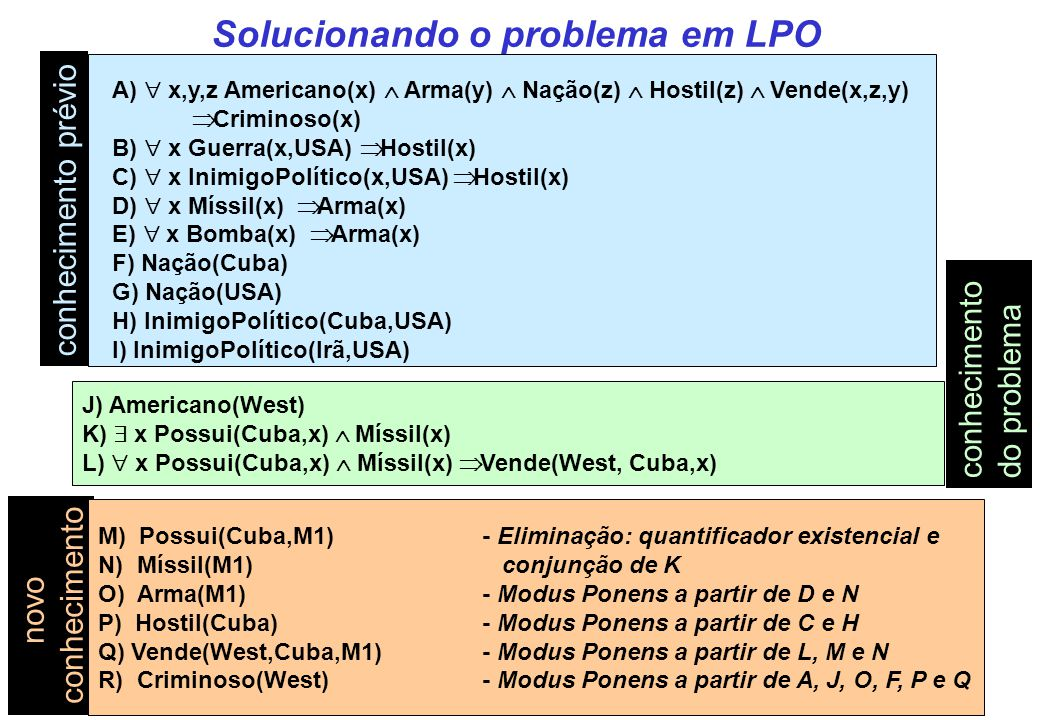
\includegraphics[scale=0.5]{figuras/exercicio_logica_01.jpg}
 \caption{Parte 2 do Exercício 3}
 \label{fig_01}
\end{figure}



\end{document}
